\chapter{Proposta de Ferramenta}

Nesta seção, será apresentada uma ferramenta cujo objetivo é automatizar a geração de questões, com o objetivo de tornar mais fácil a construção e geração de questões. A ferramenta baseia-se em um modelo de separação entre duas entidades principais : (i) um JSON de template, responsável por definir a estrutura geral das questões; e (ii) um JSON de questões, que instancia as variações específicas de cada problema. O sistema foi planejado para permitir que os professores sejam responsáveis pela elaboração e manutenção dos templates. Por outro l ado os usuários estudantes interagem apenas com as questões geradas a partir desses templates.

\section{JSON de Templates}

lolita

\begin{figure}[ht]
	\centering
	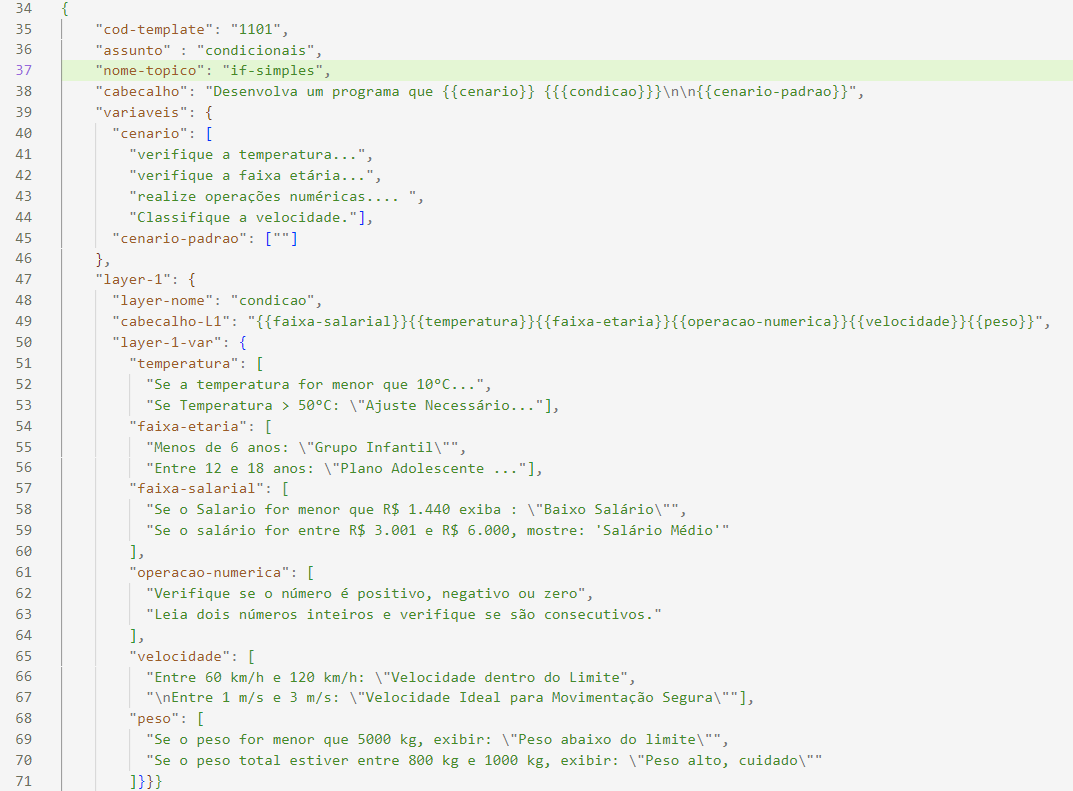
\includegraphics[width=14cm]{./imagens/capitulo7/json-de-template}
	\caption{BPMN do Fluxo de Trabalho (Autoria Propria, 2025) }
	\label{fig:bpmn-fluxo}
\end{figure}
\section{JSON de Questões}


\section{Ferramenta}